\documentclass[preprint,showpacs,amssymb,aps]{revtex4}
\usepackage{graphicx}
 
\begin{document}
\title{The near sighted principle in acheiving scalable parallelism for linear scaling first-principles calculations
%Preserving spatial locality of atoms in first-principles calculations
}
\author{Chee~K.~Gan and Matt~Challacombe
}
\affiliation{
Los Alamos National Laboratory, Theoretical Division, Group T-12, MS
B268, Los Alamos, NM 87545, USA
}
 
\begin{abstract}
A first approach to computing space filling curves with improved long-range 
properties is presented and used to solve the bandwidth problem in linear scaling 
electronic structure theory.  For matrices with elements that fall off to zero 
with geometric seperation (the near sighted principle) reordering with the new space 
filling curve yields a banded matrix with envelope reduction that is far better 
than Hilbert or Morton ordering.  This is a key problem in many fields where geometric 
seperation can be exploited to achieve scalable parallelism, but graph theory does not 
apply, is too expensive, or fails altogether.

\pacs{71.15.-m,71.15.Dx}
\end{abstract}
\maketitle


In recent years there has been substantial progress in linear scaling electronic structure methods
that achieve a reduced $O(N)$ computational cost with system size $N$, such that several programs
\cite{SIESTA,MONDO,Gaussian,?} are now able to routinely perform high quality calculations on thousands of atoms.
These $O$($N$) methods achieve reduced computational complexity by exploiting the locality of quantum 
interactions, the so called ``near sighted'' principle \cite{Kohn_96v76}.  However, in addition to 
achieving linear scaling, this principle also holds the promise for truely scalable parallel 
electronic structure algorithms.   It is this second, largely overlooked aspect of the near sighted
principle that we address here. In this work we address this second,  largely overlooked aspect of the 
near-sighted principle.   In particular, we consider the ordering of atoms in a large system for 
first-principles electronic structure calculations.   The aim is to rearrange the atoms to maximize spatial 
locality, thereby reducing the bandwidth of matrices such as the overlap,  Hamiltonian, and density matrices. 
It is then possible to exploit this property in the design of algorithms with $O(1)$ communications costs.  

Current ordering schemes involve graph theory, such as the the reverse Cuthill-McKee 
algorithm\cite{Cuthill_69,Colombo_96v37}, or geometric algorithms based on variations of
the space-filling curve (SFC) \cite{Sagan_94}.  Space-filling curves attemp to map points in space
onto a line (the SFC) such that points close in space are also close on the line.  The SFC methods 
include the Hilbert\cite{Bially_69v15,Challacombe_00v128} and Morton (also known as $Z$) 
orderings\cite{Warren_95v87,Omeltchenko_00v131}, as well as the the ``x, y, z'' ordering\cite{Canning_96v94}.  
Graph theoretic methods are very power full when addressing a single graph.  However, many electronic 
structure algorithms compute matrix-matrix products involving matrices with quite disparate graphs 
\cite{Challacombe,Hutter,Scuseria}.  Graph theory can also result in poor aspect ratios (non-uniform bandwidth), 
and can lead to widely different orderings with small perturbations.  On the other hand, current geometric 
algorithms suffer from ``loopback'', in which  two points close in space can sometimes be well separated 
(in terms of their indices) from one another in an ordered list\cite{Perez_92,Gotsman_96v5}. If localized 
atom-centered basis functions such as Gaussians are used in an electronic structure calculation, this loopback 
problem results in significant nonzero off-diagonal overlap matrix elements which are far from the main diagonal, 
increasing the bandwidth. 

In this letter, we propose a geometric ordering scheme that avoids the loopback problem, achieving superior 
``long range locality'' and band width reduction (BWR), while sacrificing ``short range locality''.  

method to efficiently reorder the atoms so that two atoms which are close to one another in space will naturally come close in an 
ordered list, so that the number of non-zero off-diagonal matrix elements
can be reduced significantly, thereby reducing the bandwidth of the matrix.

This method relies on an ordering, called the bandwidth reduction (BWR)
ordering in this work, which visits $L^3$ points in a regular 3-dimensional
grid in a certain order that spatial locality is preserved.
After obtaining a good BWR ordering $T$,
we then use $T$
to order atoms in other systems 
where the atomic positions may be irregular in space. 
This is achieved easily\cite{Warren_95v87,Pilkington_96v7}
by assigning a unique key for each atom in the system 
according $T$,
and then sort the keys to obtain an ordering of the atoms.
In what follows we shall concentrate 
on how to obtain a BWR ordering $T$ of $L^3$ points.



We consider a three-dimensional cube with $ N = L^3$ points where the position
of a grid point is given by
$(i,j,k)$ where $ 0 \le i < L$, $0 \le j < L$, and $0 \le k < L$.
We want to find an ordering, called a BWR ordering,
which visits all $N$ points in such a way that
points which are close in space will not have indices which are far apart
in the ordered list. This ordered list keeps track of
what is the first, the second, \ldots, and the $N$th point to visit.
We represent an arbitrary ordering by $P$ such that if
$P(m) = n$, then the $m$th point in the ordered list has a position
${\bf R}_n$. 
To achieve the aim we set forth earlier,
we propose an objective function called the energy which is given by
\begin{equation}
E({P}) = \frac{\alpha}{D} \sum_{i=1}^{N-1} d_{i,i+1}
+ \sum_{i=1}^{N}\sum_{j>i}
 \exp{\left( \frac{\beta |i-j| D}{N d_{i,j}}\right)},
\label{eq:objective}
\end{equation}
where $\alpha$ and $\beta$ are dimensionless non-negative constants, and
\begin{equation}
d_{i,j} = | {\bf R}_{P(i)} - {\bf R}_{P(j)} | ,
\end{equation}
which is the Euclidean distance 
between the $i$th and $j$th points in the ordered list.
$D = d_{1,N}$
is the distance between the first and the last points in the ordered 
list. We have made a simple
choice where the first and the last points
are fixed at $(0,0,0)$ and $(L-1,L-1,L-1)$, respectively.
The first single-summation 
term on the RHS of Eq.~(\ref{eq:objective})
comes from the conventional 
traveling salesman problem\cite{Press_86}, 
where the Euclidean distance between two consecutive points in an ordered list
should be as close as possible. 
The appearance of the second 
double-summation term on the RHS of Eq.~(\ref{eq:objective})
can be argued as follows. If the $i$th and $j$th points in an ordered list
have a large index separation (i.e. 
$|i-j|$ is large),
then the contribution of these two points to the energy $E$
will be large if the 
Euclidean distance between these two points ($d_{i,j}$ ) is
small. The exponential factor is used to severely penalize an ordering
with pairs of points with a large $|i-j|$ and yet a small $d_{i,j}$. 
An ordering which minimizes the energy $E$ 
will be the one which does not have physically close 
points scattered randomly in an ordered list, but more or less clustered 
together.
We note it is possible to use other objective functions besides
Eq.~(\ref{eq:objective}). 
We have replaced the exponential factor in Eq.~(\ref{eq:objective}) 
from $\beta|i-j|D/(N d_{i,j})$ to $\beta(|i-j|D/(N d_{i,j}))^2$ and
very similar results have been obtained.
In this work, we mainly use Eq.~(\ref{eq:objective}) for its simplicity.

We employ a standard simulated annealing technique\cite{Press_86} 
to obtain an optimal ordering which minimizes
the objective function. During the annealing process,
new random orderings are created using the standard recipe used to
solve the traveling salesman problem\cite{Lin_65v44,Press_86}.
When a new ordering is created, 
the energy difference $\Delta E$ is calculated between the new
and current orderings. The new ordering is then 
accepted with a probability of
$\min(1, \exp(-\Delta E/T))$, where $T$ is a temperature. Due to
the $O(N^2)$  terms in Eq.~(\ref{eq:objective}) that must be 
summed, we use a reasonably large system with $L=8$. Initially
5000 random orderings are created and $(\Delta E)_{\mbox{max}}$, the
maximum increment of energy between two consecutive orderings is recorded.
The simulated annealing process starts with
$T$ set to $(\Delta E)_{\mbox{max}}/2$. At most $100N$ random orderings
are tried for each temperature. An annealing process is achieved by
reducing $T$ by a factor of 0.9 from its original value.
The annealing process is stopped
when the acceptance of the proposed moves is 
reasonably small (such as 0.5\%).
We have performed calculations 
for a range of $\alpha$ and $\beta$.

To quantify the locality of each of the ordering $P$ we obtained, 
a measure $C$ is defined by
\begin{equation}
C(P) = \max_{j>i} v_{i,j} ,
\end{equation} 
where $v_{i,j} =  |i-j|/d_{i,j} $.
%Generally, for a certain value of $\beta$, we find 
%that nonzero values of $\alpha$ do not improve $C$ much.
%Therefore for convenience, we usually make $\alpha=0$.
The values of $C$ for the Hilbert and Morton orderings 
on a $8\times 8 \times 8$ regular grid 
are 475.0 and 233.3, respectively.
However, with $\alpha=0$ and $\beta=1.0$, the ordering we generated 
has $C$ equals to 102.0, which is 4.7 and 2.3 times smaller than the
Hilbert and Morton orderings, respectively.
We note that for a particular value of $\beta$, non-zero values of $\alpha$ 
do not improve the value of $C$. This means the effect of double-summation 
term (which involves $O(N^2)$ terms) in Eq.~(\ref{eq:objective}) 
is stronger than the single-summation term (which involves $O(N)$ terms)
to determine the value of $C$. 
To better illustrate the locality-preserving 
property of these three orderings,
we calculate the frequency
plot of $v_{i,j}$ and the results are 
shown in Fig.~\ref{fig:compare_all}. It is observed that 
the Hilbert ordering 
has a peak for small values of $v_{i,j}$. 
Unfortunately, 
the curve decays very slowly to zero, where $v_{i,j}$ extends all the way
to 475.0.
Without the long tail, Hilbert ordering 
could have been the best ordering among these
three orderings.
It is observed that the curve corresponds to our BWR ordering goes 
to zero very abruptly for 
values of $v_{i,j}$ starting around 50.

To illustrate the efficiency of the BWR ordering, 
we investigate the sparsity pattern of 
the overlap matrix $S$ of a system of 
350 water molecules with atom-centered Gaussian basis functions
using the Hilbert, Morton, and BWR orderings, which are 
shown in 
Figs.~\ref{fig:hilbert_s}, \ref{fig:morton_s}, and
~\ref{fig:anneal_s}, respectively.
Each dot in the figure corresponds to a non-zero submatrix
created by the substantial overlap of
two groups of atom-centered Gaussian basis functions.
It is clearly seen that 
the bandwidth of $S$ has been greatly reduced using our BWR ordering.
It is interesting to note that 
there are three distinct bands parallel to the main diagonal in the sparsity
pattern obtained with the BWR ordering.
The empty space between these bands is caused by basis functions in 
blocks of atoms which 
do not overlap significantly with basis functions 
in other blocks of atoms. These blocks of atoms
are created when the whole 350 water molecule system is 
divided up into $8^3$ cubes. 
Since the value of $L$ (which is 8) we used
is slightly smaller with respect to the water molecule system that we have used, 
the block of atoms created are
fairly large. One way to reduce or remove the spacing between the 
bands is to use a BWR ordering obtained from a system 
with a larger $L$. We have found the the 
band spacing is indeed substantially larger
when a BWR ordering with $L=6$ is used, as expected.

In summary we have proposed a new novel method to reorder atoms which 
preserves the spatial locality of the atoms.
In view of the facts that locality preserving ordering is 
very important in many applications such as the domain decomposition of the
$N$-body problem~\cite{Warren_95v87} and 
improvement of memory hierarchy performance~\cite{Mellor-Crummey_01v29},
we believe that the BWR ordering should not be restricted
to the field of first-principles calculations.
It is important to point out that systems with large $L$ should be 
simulated to obtain orderings which can optimally 
preserve the spatial locality 
of very large systems.
Finally it should be noted that one may use Eq.~(\ref{eq:objective}) 
directly to perform a simulated annealing to reorder all 
atoms in a system containing many atoms. 
However, this might not be practical
since the time taken to perform the simulated annealing will be 
very long.

\bibliographystyle{plain}
\begin{thebibliography}{10}

\bibitem{Goedecker_99v71}
S. Goedecker, Rev. Mod. Phys. {\bf 71},  1085  (1999).

\bibitem{Kohn_96v76}
W. Kohn, Phys. Rev. Lett. {\bf 76},  3168  (1996).

\bibitem{Colombo_96v37}
L. Colombo and W. Sawyer, Mat. Sci. Eng. B {\bf 37},  228  (1996).

\bibitem{Cuthill_69}
E.~H. Cuthill and J. McKee, Proc. 24th Natl. Conf. Assoc. Comp. Mach. ACM  157
  (1969).

\bibitem{Sagan_94}
H. Sagan, {\em Space-filling curves} (Universitext, Springer Verlag, 1994).

\bibitem{Bially_69v15}
T. Bially, IEEE Trans. Inf. Th. {\bf 15},  658  (1969).

\bibitem{Challacombe_00v128}
M. Challacombe, Comput. Phys. Commun. {\bf 128},  93  (2000).

\bibitem{Omeltchenko_00v131}
A. Omeltchenko {\it et~al.}, Comput. Phys. Commun. {\bf 131},  78  (2000).

\bibitem{Warren_95v87}
M.~S. Warren and J.~K. Salmon, Comput. Phys. Commun. {\bf 87},  266  (1995).

\bibitem{Canning_96v94}
A. Canning {\it et~al.}, Comput. Phys. Commun. {\bf 94},  89  (1996).

\bibitem{Perez_92}
A. P\'{e}rez, S. Kamata, and E. Kawaguchi, Proc. 11th IAPR Int. Conf. Patt.
  Recogn.  565  (1992).

\bibitem{Gotsman_96v5}
C. Gotsman and M. Lindenbaum, IEEE Trans. Image Proc. {\bf 5},  794  (1996).

\bibitem{Pilkington_96v7}
J.~R. Pilkington and S. Baden, IEEE Trans. Para. Dist. Sys. {\bf 1996},  288
  (1996).

\bibitem{Press_86}
W. Press, B.~P. Flannery, S.~A. Teukolsky, and W.~T. Vetterling, {\em Numerical
  Recipes, the Art of Scientific Computing} (Cambridge University Press,
  Cambridge, England, 1986).

\bibitem{Lin_65v44}
L. S., Bell Sys. Tech. J. {\bf 44},  2245  (1965).

\bibitem{Mellor-Crummey_01v29}
J. Mellor-Crummey, D. Whalley, and K. Kennedy, Int. J. Para. Comp. {\bf 29},
  217  (2001).

\end{thebibliography}

\begin{figure}
{\includegraphics[width=8cm]{compare_all.eps}}
\caption{The frequency plots of $v_{i,j} = |i-j|/d_{i,j}$ for
three different orderings.
}
\label{fig:compare_all}
\end{figure} 

\begin{figure}
{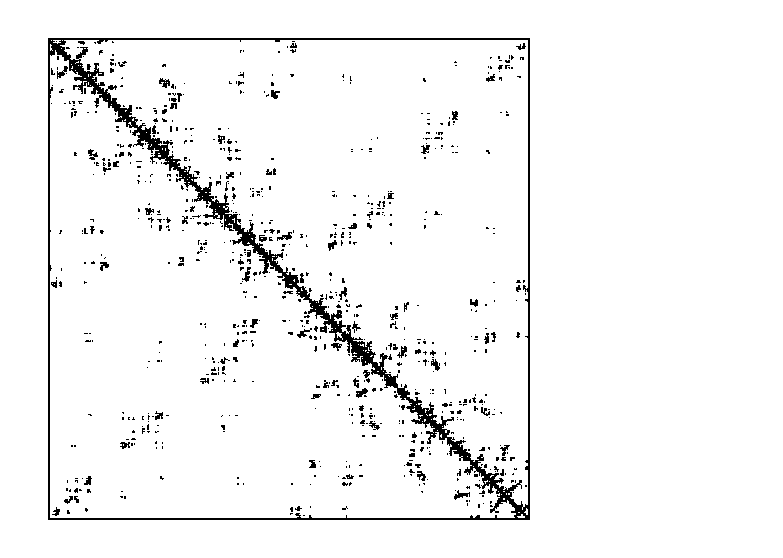
\includegraphics[width=8cm]{hilbert_s.eps}}
\caption{Sparsity pattern of $S$ using the Hilbert ordering.
}
\label{fig:hilbert_s}
\end{figure} 

\begin{figure}
{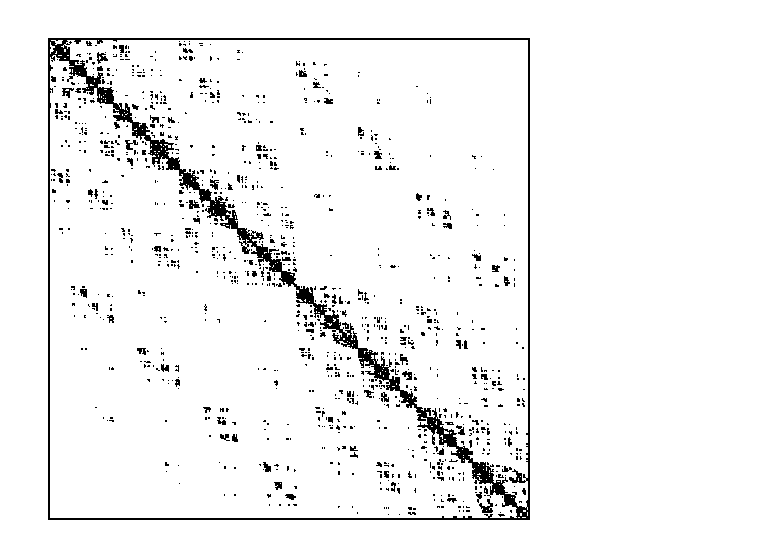
\includegraphics[width=8cm]{morton_s.eps}}
\caption{
Sparsity pattern of $S$ using the Morton ordering.
}
\label{fig:morton_s}
\end{figure} 

\begin{figure}
{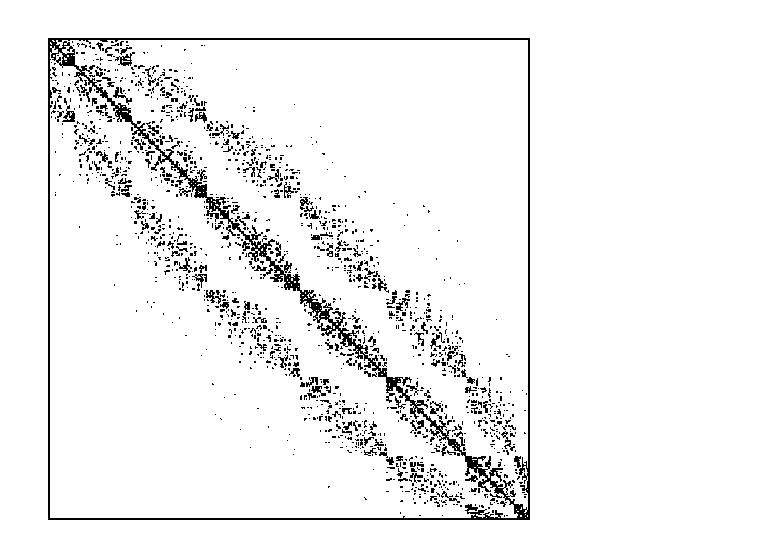
\includegraphics[width=8cm]{anneal_s.eps}}
\caption{
Sparsity pattern of $S$ using the BWR ordering, with
$\alpha=0$ and $\beta = 1.0$.
}
\label{fig:anneal_s}
\end{figure} 

\end{document}
